% Created by tikzDevice version 0.10.1 on 2018-01-19 13:04:00
% !TEX encoding = UTF-8 Unicode
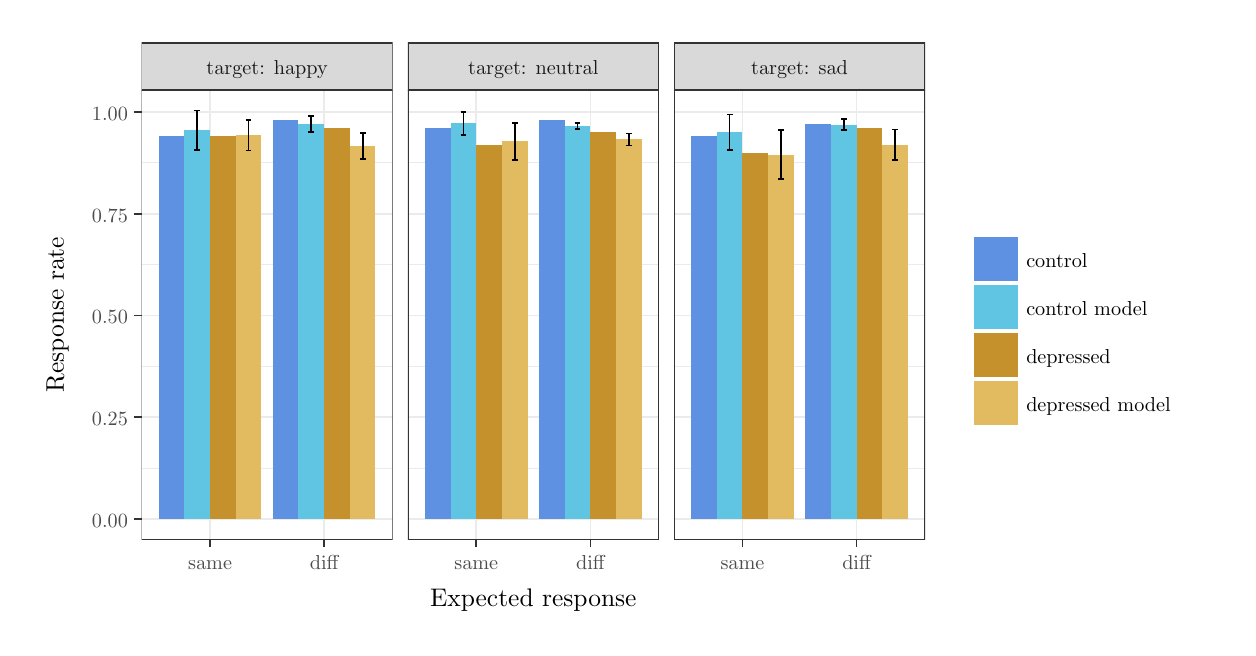
\begin{tikzpicture}[x=1pt,y=1pt]
\definecolor{fillColor}{RGB}{255,255,255}
\path[use as bounding box,fill=fillColor,fill opacity=0.00] (0,0) rectangle (433.62,216.81);
\begin{scope}
\path[clip] (  0.00,  0.00) rectangle (433.62,216.81);
\definecolor{drawColor}{RGB}{255,255,255}
\definecolor{fillColor}{RGB}{255,255,255}

\path[draw=drawColor,line width= 0.6pt,line join=round,line cap=round,fill=fillColor] (  0.00,  0.00) rectangle (433.62,216.81);
\end{scope}
\begin{scope}
\path[clip] ( 41.17, 31.92) rectangle (131.87,194.25);
\definecolor{fillColor}{RGB}{255,255,255}

\path[fill=fillColor] ( 41.17, 31.92) rectangle (131.87,194.25);
\definecolor{drawColor}{gray}{0.92}

\path[draw=drawColor,line width= 0.3pt,line join=round] ( 41.17, 57.68) --
	(131.87, 57.68);

\path[draw=drawColor,line width= 0.3pt,line join=round] ( 41.17, 94.43) --
	(131.87, 94.43);

\path[draw=drawColor,line width= 0.3pt,line join=round] ( 41.17,131.19) --
	(131.87,131.19);

\path[draw=drawColor,line width= 0.3pt,line join=round] ( 41.17,167.94) --
	(131.87,167.94);

\path[draw=drawColor,line width= 0.6pt,line join=round] ( 41.17, 39.30) --
	(131.87, 39.30);

\path[draw=drawColor,line width= 0.6pt,line join=round] ( 41.17, 76.05) --
	(131.87, 76.05);

\path[draw=drawColor,line width= 0.6pt,line join=round] ( 41.17,112.81) --
	(131.87,112.81);

\path[draw=drawColor,line width= 0.6pt,line join=round] ( 41.17,149.57) --
	(131.87,149.57);

\path[draw=drawColor,line width= 0.6pt,line join=round] ( 41.17,186.32) --
	(131.87,186.32);

\path[draw=drawColor,line width= 0.6pt,line join=round] ( 65.91, 31.92) --
	( 65.91,194.25);

\path[draw=drawColor,line width= 0.6pt,line join=round] (107.13, 31.92) --
	(107.13,194.25);
\definecolor{fillColor}{RGB}{226,186,95}

\path[fill=fillColor] ( 75.18, 39.30) rectangle ( 84.46,177.87);
\definecolor{fillColor}{RGB}{196,145,45}

\path[fill=fillColor] ( 65.91, 39.30) rectangle ( 75.18,177.50);
\definecolor{fillColor}{RGB}{95,197,226}

\path[fill=fillColor] ( 56.63, 39.30) rectangle ( 65.91,179.71);
\definecolor{fillColor}{RGB}{95,145,226}

\path[fill=fillColor] ( 47.36, 39.30) rectangle ( 56.63,177.50);
\definecolor{fillColor}{RGB}{226,186,95}

\path[fill=fillColor] (116.41, 39.30) rectangle (125.68,174.10);
\definecolor{fillColor}{RGB}{196,145,45}

\path[fill=fillColor] (107.13, 39.30) rectangle (116.41,180.44);
\definecolor{fillColor}{RGB}{95,197,226}

\path[fill=fillColor] ( 97.86, 39.30) rectangle (107.13,182.05);
\definecolor{fillColor}{RGB}{95,145,226}

\path[fill=fillColor] ( 88.58, 39.30) rectangle ( 97.86,183.38);
\definecolor{drawColor}{RGB}{0,0,0}

\path[draw=drawColor,line width= 0.6pt,line join=round] ( 78.79,183.37) --
	( 80.85,183.37);

\path[draw=drawColor,line width= 0.6pt,line join=round] ( 79.82,183.37) --
	( 79.82,172.37);

\path[draw=drawColor,line width= 0.6pt,line join=round] ( 78.79,172.37) --
	( 80.85,172.37);

\path[draw=drawColor,line width= 0.6pt,line join=round] ( 60.24,186.87) --
	( 62.30,186.87);

\path[draw=drawColor,line width= 0.6pt,line join=round] ( 61.27,186.87) --
	( 61.27,172.54);

\path[draw=drawColor,line width= 0.6pt,line join=round] ( 60.24,172.54) --
	( 62.30,172.54);

\path[draw=drawColor,line width= 0.6pt,line join=round] (120.01,178.80) --
	(122.08,178.80);

\path[draw=drawColor,line width= 0.6pt,line join=round] (121.05,178.80) --
	(121.05,169.41);

\path[draw=drawColor,line width= 0.6pt,line join=round] (120.01,169.41) --
	(122.08,169.41);

\path[draw=drawColor,line width= 0.6pt,line join=round] (101.46,184.90) --
	(103.52,184.90);

\path[draw=drawColor,line width= 0.6pt,line join=round] (102.49,184.90) --
	(102.49,179.19);

\path[draw=drawColor,line width= 0.6pt,line join=round] (101.46,179.19) --
	(103.52,179.19);
\definecolor{drawColor}{gray}{0.20}

\path[draw=drawColor,line width= 0.6pt,line join=round,line cap=round] ( 41.17, 31.92) rectangle (131.87,194.25);
\end{scope}
\begin{scope}
\path[clip] (137.37, 31.92) rectangle (228.06,194.25);
\definecolor{fillColor}{RGB}{255,255,255}

\path[fill=fillColor] (137.37, 31.92) rectangle (228.06,194.25);
\definecolor{drawColor}{gray}{0.92}

\path[draw=drawColor,line width= 0.3pt,line join=round] (137.37, 57.68) --
	(228.06, 57.68);

\path[draw=drawColor,line width= 0.3pt,line join=round] (137.37, 94.43) --
	(228.06, 94.43);

\path[draw=drawColor,line width= 0.3pt,line join=round] (137.37,131.19) --
	(228.06,131.19);

\path[draw=drawColor,line width= 0.3pt,line join=round] (137.37,167.94) --
	(228.06,167.94);

\path[draw=drawColor,line width= 0.6pt,line join=round] (137.37, 39.30) --
	(228.06, 39.30);

\path[draw=drawColor,line width= 0.6pt,line join=round] (137.37, 76.05) --
	(228.06, 76.05);

\path[draw=drawColor,line width= 0.6pt,line join=round] (137.37,112.81) --
	(228.06,112.81);

\path[draw=drawColor,line width= 0.6pt,line join=round] (137.37,149.57) --
	(228.06,149.57);

\path[draw=drawColor,line width= 0.6pt,line join=round] (137.37,186.32) --
	(228.06,186.32);

\path[draw=drawColor,line width= 0.6pt,line join=round] (162.10, 31.92) --
	(162.10,194.25);

\path[draw=drawColor,line width= 0.6pt,line join=round] (203.33, 31.92) --
	(203.33,194.25);
\definecolor{fillColor}{RGB}{226,186,95}

\path[fill=fillColor] (171.38, 39.30) rectangle (180.65,175.70);
\definecolor{fillColor}{RGB}{196,145,45}

\path[fill=fillColor] (162.10, 39.30) rectangle (171.38,174.56);
\definecolor{fillColor}{RGB}{95,197,226}

\path[fill=fillColor] (152.83, 39.30) rectangle (162.10,182.21);
\definecolor{fillColor}{RGB}{95,145,226}

\path[fill=fillColor] (143.55, 39.30) rectangle (152.83,180.44);
\definecolor{fillColor}{RGB}{226,186,95}

\path[fill=fillColor] (212.60, 39.30) rectangle (221.88,176.40);
\definecolor{fillColor}{RGB}{196,145,45}

\path[fill=fillColor] (203.33, 39.30) rectangle (212.60,178.97);
\definecolor{fillColor}{RGB}{95,197,226}

\path[fill=fillColor] (194.05, 39.30) rectangle (203.33,181.17);
\definecolor{fillColor}{RGB}{95,145,226}

\path[fill=fillColor] (184.77, 39.30) rectangle (194.05,183.38);
\definecolor{drawColor}{RGB}{0,0,0}

\path[draw=drawColor,line width= 0.6pt,line join=round] (174.98,182.48) --
	(177.04,182.48);

\path[draw=drawColor,line width= 0.6pt,line join=round] (176.01,182.48) --
	(176.01,168.92);

\path[draw=drawColor,line width= 0.6pt,line join=round] (174.98,168.92) --
	(177.04,168.92);

\path[draw=drawColor,line width= 0.6pt,line join=round] (156.43,186.44) --
	(158.49,186.44);

\path[draw=drawColor,line width= 0.6pt,line join=round] (157.46,186.44) --
	(157.46,177.98);

\path[draw=drawColor,line width= 0.6pt,line join=round] (156.43,177.98) --
	(158.49,177.98);

\path[draw=drawColor,line width= 0.6pt,line join=round] (216.21,178.51) --
	(218.27,178.51);

\path[draw=drawColor,line width= 0.6pt,line join=round] (217.24,178.51) --
	(217.24,174.29);

\path[draw=drawColor,line width= 0.6pt,line join=round] (216.21,174.29) --
	(218.27,174.29);

\path[draw=drawColor,line width= 0.6pt,line join=round] (197.66,182.27) --
	(199.72,182.27);

\path[draw=drawColor,line width= 0.6pt,line join=round] (198.69,182.27) --
	(198.69,180.08);

\path[draw=drawColor,line width= 0.6pt,line join=round] (197.66,180.08) --
	(199.72,180.08);
\definecolor{drawColor}{gray}{0.20}

\path[draw=drawColor,line width= 0.6pt,line join=round,line cap=round] (137.37, 31.92) rectangle (228.06,194.25);
\end{scope}
\begin{scope}
\path[clip] (233.56, 31.92) rectangle (324.25,194.25);
\definecolor{fillColor}{RGB}{255,255,255}

\path[fill=fillColor] (233.56, 31.92) rectangle (324.25,194.25);
\definecolor{drawColor}{gray}{0.92}

\path[draw=drawColor,line width= 0.3pt,line join=round] (233.56, 57.68) --
	(324.25, 57.68);

\path[draw=drawColor,line width= 0.3pt,line join=round] (233.56, 94.43) --
	(324.25, 94.43);

\path[draw=drawColor,line width= 0.3pt,line join=round] (233.56,131.19) --
	(324.25,131.19);

\path[draw=drawColor,line width= 0.3pt,line join=round] (233.56,167.94) --
	(324.25,167.94);

\path[draw=drawColor,line width= 0.6pt,line join=round] (233.56, 39.30) --
	(324.25, 39.30);

\path[draw=drawColor,line width= 0.6pt,line join=round] (233.56, 76.05) --
	(324.25, 76.05);

\path[draw=drawColor,line width= 0.6pt,line join=round] (233.56,112.81) --
	(324.25,112.81);

\path[draw=drawColor,line width= 0.6pt,line join=round] (233.56,149.57) --
	(324.25,149.57);

\path[draw=drawColor,line width= 0.6pt,line join=round] (233.56,186.32) --
	(324.25,186.32);

\path[draw=drawColor,line width= 0.6pt,line join=round] (258.29, 31.92) --
	(258.29,194.25);

\path[draw=drawColor,line width= 0.6pt,line join=round] (299.52, 31.92) --
	(299.52,194.25);
\definecolor{fillColor}{RGB}{226,186,95}

\path[fill=fillColor] (267.57, 39.30) rectangle (276.85,170.96);
\definecolor{fillColor}{RGB}{196,145,45}

\path[fill=fillColor] (258.29, 39.30) rectangle (267.57,171.62);
\definecolor{fillColor}{RGB}{95,197,226}

\path[fill=fillColor] (249.02, 39.30) rectangle (258.29,179.04);
\definecolor{fillColor}{RGB}{95,145,226}

\path[fill=fillColor] (239.74, 39.30) rectangle (249.02,177.50);
\definecolor{fillColor}{RGB}{226,186,95}

\path[fill=fillColor] (308.79, 39.30) rectangle (318.07,174.56);
\definecolor{fillColor}{RGB}{196,145,45}

\path[fill=fillColor] (299.52, 39.30) rectangle (308.79,180.44);
\definecolor{fillColor}{RGB}{95,197,226}

\path[fill=fillColor] (290.24, 39.30) rectangle (299.52,181.79);
\definecolor{fillColor}{RGB}{95,145,226}

\path[fill=fillColor] (280.97, 39.30) rectangle (290.24,181.91);
\definecolor{drawColor}{RGB}{0,0,0}

\path[draw=drawColor,line width= 0.6pt,line join=round] (271.18,179.88) --
	(273.24,179.88);

\path[draw=drawColor,line width= 0.6pt,line join=round] (272.21,179.88) --
	(272.21,162.03);

\path[draw=drawColor,line width= 0.6pt,line join=round] (271.18,162.03) --
	(273.24,162.03);

\path[draw=drawColor,line width= 0.6pt,line join=round] (252.63,185.47) --
	(254.69,185.47);

\path[draw=drawColor,line width= 0.6pt,line join=round] (253.66,185.47) --
	(253.66,172.61);

\path[draw=drawColor,line width= 0.6pt,line join=round] (252.63,172.61) --
	(254.69,172.61);

\path[draw=drawColor,line width= 0.6pt,line join=round] (312.40,180.07) --
	(314.46,180.07);

\path[draw=drawColor,line width= 0.6pt,line join=round] (313.43,180.07) --
	(313.43,169.05);

\path[draw=drawColor,line width= 0.6pt,line join=round] (312.40,169.05) --
	(314.46,169.05);

\path[draw=drawColor,line width= 0.6pt,line join=round] (293.85,183.84) --
	(295.91,183.84);

\path[draw=drawColor,line width= 0.6pt,line join=round] (294.88,183.84) --
	(294.88,179.74);

\path[draw=drawColor,line width= 0.6pt,line join=round] (293.85,179.74) --
	(295.91,179.74);
\definecolor{drawColor}{gray}{0.20}

\path[draw=drawColor,line width= 0.6pt,line join=round,line cap=round] (233.56, 31.92) rectangle (324.25,194.25);
\end{scope}
\begin{scope}
\path[clip] ( 41.17,194.25) rectangle (131.87,211.31);
\definecolor{drawColor}{gray}{0.20}
\definecolor{fillColor}{gray}{0.85}

\path[draw=drawColor,line width= 0.6pt,line join=round,line cap=round,fill=fillColor] ( 41.17,194.25) rectangle (131.87,211.31);
\definecolor{drawColor}{gray}{0.10}

\node[text=drawColor,anchor=base,inner sep=0pt, outer sep=0pt, scale=  0.73] at ( 86.52,199.75) {target: happy};
\end{scope}
\begin{scope}
\path[clip] (137.37,194.25) rectangle (228.06,211.31);
\definecolor{drawColor}{gray}{0.20}
\definecolor{fillColor}{gray}{0.85}

\path[draw=drawColor,line width= 0.6pt,line join=round,line cap=round,fill=fillColor] (137.37,194.25) rectangle (228.06,211.31);
\definecolor{drawColor}{gray}{0.10}

\node[text=drawColor,anchor=base,inner sep=0pt, outer sep=0pt, scale=  0.73] at (182.71,199.75) {target: neutral};
\end{scope}
\begin{scope}
\path[clip] (233.56,194.25) rectangle (324.25,211.31);
\definecolor{drawColor}{gray}{0.20}
\definecolor{fillColor}{gray}{0.85}

\path[draw=drawColor,line width= 0.6pt,line join=round,line cap=round,fill=fillColor] (233.56,194.25) rectangle (324.25,211.31);
\definecolor{drawColor}{gray}{0.10}

\node[text=drawColor,anchor=base,inner sep=0pt, outer sep=0pt, scale=  0.73] at (278.91,199.75) {target: sad};
\end{scope}
\begin{scope}
\path[clip] (  0.00,  0.00) rectangle (433.62,216.81);
\definecolor{drawColor}{gray}{0.20}

\path[draw=drawColor,line width= 0.6pt,line join=round] ( 65.91, 29.17) --
	( 65.91, 31.92);

\path[draw=drawColor,line width= 0.6pt,line join=round] (107.13, 29.17) --
	(107.13, 31.92);
\end{scope}
\begin{scope}
\path[clip] (  0.00,  0.00) rectangle (433.62,216.81);
\definecolor{drawColor}{gray}{0.30}

\node[text=drawColor,anchor=base,inner sep=0pt, outer sep=0pt, scale=  0.73] at ( 65.91, 20.91) {same};

\node[text=drawColor,anchor=base,inner sep=0pt, outer sep=0pt, scale=  0.73] at (107.13, 20.91) {diff};
\end{scope}
\begin{scope}
\path[clip] (  0.00,  0.00) rectangle (433.62,216.81);
\definecolor{drawColor}{gray}{0.20}

\path[draw=drawColor,line width= 0.6pt,line join=round] (162.10, 29.17) --
	(162.10, 31.92);

\path[draw=drawColor,line width= 0.6pt,line join=round] (203.33, 29.17) --
	(203.33, 31.92);
\end{scope}
\begin{scope}
\path[clip] (  0.00,  0.00) rectangle (433.62,216.81);
\definecolor{drawColor}{gray}{0.30}

\node[text=drawColor,anchor=base,inner sep=0pt, outer sep=0pt, scale=  0.73] at (162.10, 20.91) {same};

\node[text=drawColor,anchor=base,inner sep=0pt, outer sep=0pt, scale=  0.73] at (203.33, 20.91) {diff};
\end{scope}
\begin{scope}
\path[clip] (  0.00,  0.00) rectangle (433.62,216.81);
\definecolor{drawColor}{gray}{0.20}

\path[draw=drawColor,line width= 0.6pt,line join=round] (258.29, 29.17) --
	(258.29, 31.92);

\path[draw=drawColor,line width= 0.6pt,line join=round] (299.52, 29.17) --
	(299.52, 31.92);
\end{scope}
\begin{scope}
\path[clip] (  0.00,  0.00) rectangle (433.62,216.81);
\definecolor{drawColor}{gray}{0.30}

\node[text=drawColor,anchor=base,inner sep=0pt, outer sep=0pt, scale=  0.73] at (258.29, 20.91) {same};

\node[text=drawColor,anchor=base,inner sep=0pt, outer sep=0pt, scale=  0.73] at (299.52, 20.91) {diff};
\end{scope}
\begin{scope}
\path[clip] (  0.00,  0.00) rectangle (433.62,216.81);
\definecolor{drawColor}{gray}{0.30}

\node[text=drawColor,anchor=base east,inner sep=0pt, outer sep=0pt, scale=  0.73] at ( 36.22, 36.27) {0.00};

\node[text=drawColor,anchor=base east,inner sep=0pt, outer sep=0pt, scale=  0.73] at ( 36.22, 73.02) {0.25};

\node[text=drawColor,anchor=base east,inner sep=0pt, outer sep=0pt, scale=  0.73] at ( 36.22,109.78) {0.50};

\node[text=drawColor,anchor=base east,inner sep=0pt, outer sep=0pt, scale=  0.73] at ( 36.22,146.54) {0.75};

\node[text=drawColor,anchor=base east,inner sep=0pt, outer sep=0pt, scale=  0.73] at ( 36.22,183.29) {1.00};
\end{scope}
\begin{scope}
\path[clip] (  0.00,  0.00) rectangle (433.62,216.81);
\definecolor{drawColor}{gray}{0.20}

\path[draw=drawColor,line width= 0.6pt,line join=round] ( 38.42, 39.30) --
	( 41.17, 39.30);

\path[draw=drawColor,line width= 0.6pt,line join=round] ( 38.42, 76.05) --
	( 41.17, 76.05);

\path[draw=drawColor,line width= 0.6pt,line join=round] ( 38.42,112.81) --
	( 41.17,112.81);

\path[draw=drawColor,line width= 0.6pt,line join=round] ( 38.42,149.57) --
	( 41.17,149.57);

\path[draw=drawColor,line width= 0.6pt,line join=round] ( 38.42,186.32) --
	( 41.17,186.32);
\end{scope}
\begin{scope}
\path[clip] (  0.00,  0.00) rectangle (433.62,216.81);
\definecolor{drawColor}{RGB}{0,0,0}

\node[text=drawColor,anchor=base,inner sep=0pt, outer sep=0pt, scale=  0.92] at (182.71,  7.83) {Expected response};
\end{scope}
\begin{scope}
\path[clip] (  0.00,  0.00) rectangle (433.62,216.81);
\definecolor{drawColor}{RGB}{0,0,0}

\node[text=drawColor,rotate= 90.00,anchor=base,inner sep=0pt, outer sep=0pt, scale=  0.92] at ( 13.08,113.08) {Response rate};
\end{scope}
\begin{scope}
\path[clip] (  0.00,  0.00) rectangle (433.62,216.81);
\definecolor{fillColor}{RGB}{255,255,255}

\path[fill=fillColor] (335.63, 66.75) rectangle (428.12,159.42);
\end{scope}
\begin{scope}
\path[clip] (  0.00,  0.00) rectangle (433.62,216.81);
\definecolor{fillColor}{RGB}{255,255,255}

\path[fill=fillColor] (341.32,124.47) rectangle (358.67,141.82);
\end{scope}
\begin{scope}
\path[clip] (  0.00,  0.00) rectangle (433.62,216.81);
\definecolor{fillColor}{RGB}{95,145,226}

\path[fill=fillColor] (342.04,125.18) rectangle (357.96,141.11);
\end{scope}
\begin{scope}
\path[clip] (  0.00,  0.00) rectangle (433.62,216.81);
\definecolor{fillColor}{RGB}{255,255,255}

\path[fill=fillColor] (341.32,107.13) rectangle (358.67,124.47);
\end{scope}
\begin{scope}
\path[clip] (  0.00,  0.00) rectangle (433.62,216.81);
\definecolor{fillColor}{RGB}{95,197,226}

\path[fill=fillColor] (342.04,107.84) rectangle (357.96,123.76);
\end{scope}
\begin{scope}
\path[clip] (  0.00,  0.00) rectangle (433.62,216.81);
\definecolor{fillColor}{RGB}{255,255,255}

\path[fill=fillColor] (341.32, 89.78) rectangle (358.67,107.13);
\end{scope}
\begin{scope}
\path[clip] (  0.00,  0.00) rectangle (433.62,216.81);
\definecolor{fillColor}{RGB}{196,145,45}

\path[fill=fillColor] (342.04, 90.49) rectangle (357.96,106.42);
\end{scope}
\begin{scope}
\path[clip] (  0.00,  0.00) rectangle (433.62,216.81);
\definecolor{fillColor}{RGB}{255,255,255}

\path[fill=fillColor] (341.32, 72.44) rectangle (358.67, 89.78);
\end{scope}
\begin{scope}
\path[clip] (  0.00,  0.00) rectangle (433.62,216.81);
\definecolor{fillColor}{RGB}{226,186,95}

\path[fill=fillColor] (342.04, 73.15) rectangle (357.96, 89.07);
\end{scope}
\begin{scope}
\path[clip] (  0.00,  0.00) rectangle (433.62,216.81);
\definecolor{drawColor}{RGB}{0,0,0}

\node[text=drawColor,anchor=base west,inner sep=0pt, outer sep=0pt, scale=  0.73] at (360.84,130.12) {control};
\end{scope}
\begin{scope}
\path[clip] (  0.00,  0.00) rectangle (433.62,216.81);
\definecolor{drawColor}{RGB}{0,0,0}

\node[text=drawColor,anchor=base west,inner sep=0pt, outer sep=0pt, scale=  0.73] at (360.84,112.77) {control model};
\end{scope}
\begin{scope}
\path[clip] (  0.00,  0.00) rectangle (433.62,216.81);
\definecolor{drawColor}{RGB}{0,0,0}

\node[text=drawColor,anchor=base west,inner sep=0pt, outer sep=0pt, scale=  0.73] at (360.84, 95.43) {depressed};
\end{scope}
\begin{scope}
\path[clip] (  0.00,  0.00) rectangle (433.62,216.81);
\definecolor{drawColor}{RGB}{0,0,0}

\node[text=drawColor,anchor=base west,inner sep=0pt, outer sep=0pt, scale=  0.73] at (360.84, 78.08) {depressed model};
\end{scope}
\end{tikzpicture}
